% Chapter Template

\chapter{Basic Characteristics} % Main chapter title
In the following section, I will describe the basic characteristics of my Department’s structure and my role as an intern.
\label{Chapter2} 

\section{ Department }
The Department that I am part of is the Greek Market. Greek Market is managing the marketplace of Greece and is also referred as the Beat of Greece as mentioned in the previous chapter.

\subsection{Role in the Company}
The Greek Market is the only department focused on Greece. Its role inside the company is to manage any demands referred to this marketplace. Demands on marketing, finance, business analysis, customer experience and the development of product BeatHotels that is provided only in Greece, are all responsibility of this department.\par 
The Beat App is developed by other departments and any changes required for the greek marketplace are forwarded from the Greek Market to the Engineering Department of Beat.

\subsection{Department's structure}
Greek Market is constituted by five teams, Operations, Costumer Experience, the Engineer's of Beat Hotels named as GR Squad team, Marketing, and Finance team. The General Manager of this Department is Vasilis Danias and the total number of people working in it is 37. 
\begin{figure}[h!]
	\begin{center}
		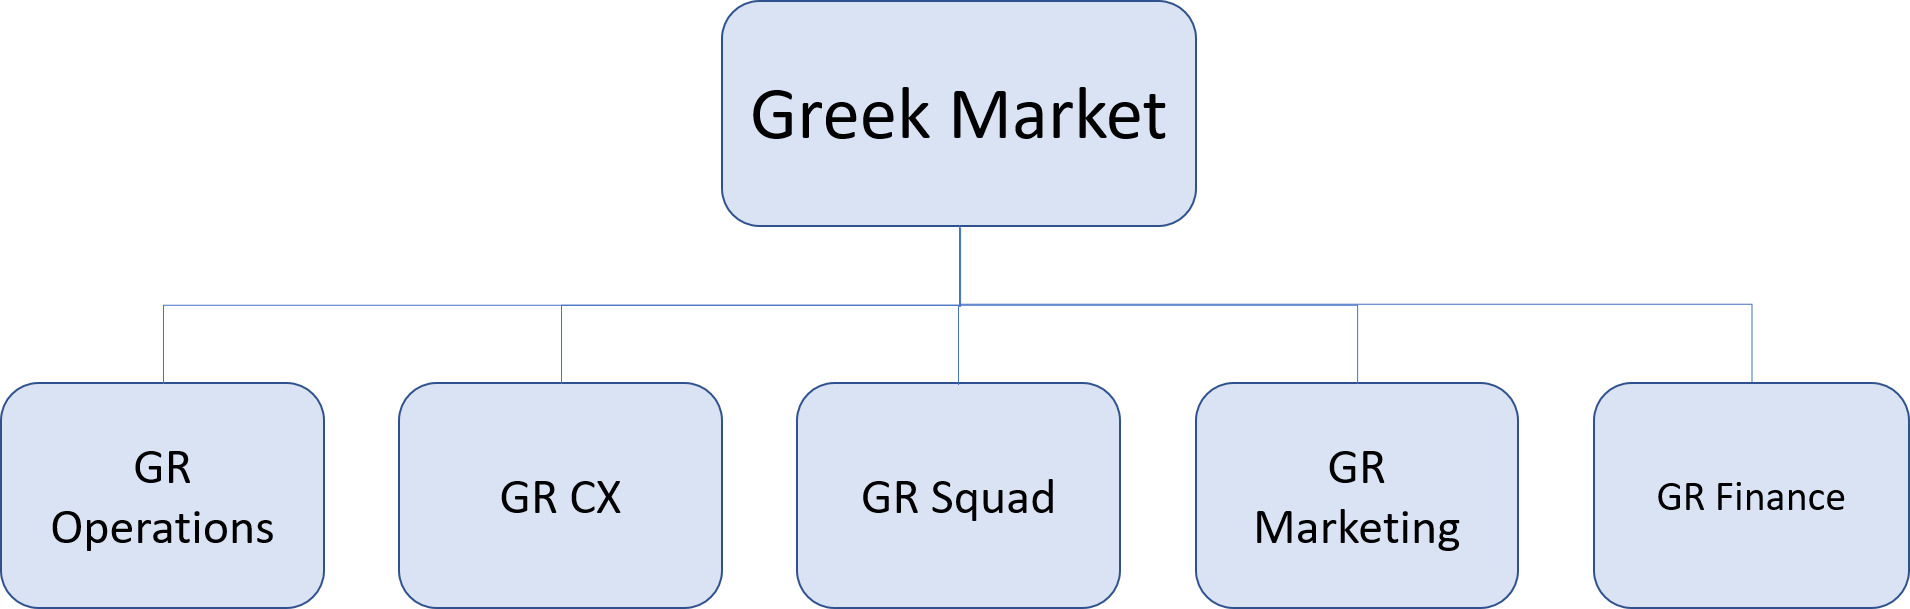
\includegraphics[scale=0.4]{images/GR_Market_structure.png}
	\end{center}
	\caption{Greek Market's structure}
\end{figure}

\subsection{Basic Procedures}
Department's basic procedures are based on the management of three products in the borders of greek market, Hive, Beat App and Beat Hotels.\par
In more detail, each team has different responsibilities. CX team is responsible for training drivers, resolving tickets and detecting any problems regarding these three products. The term tickets are any calls or visits made or emails sent by either a passenger or driver.\par 
The operations team is responsible for designing and controlling the process of production and redesigning business operations in terms of using as few resources as needed and meeting customer requirements. 
Marketing is creating, communicating, delivering, and exchanging offerings that have value for both customers and society in total. Competitions, sponsorships, banners, products or videos created for advertisement and social media management are made by this team.\par
Finance is responsible for beat driver's payments, while GR Squad is the team responsible for developing BeatHotels service.

\subsection{ GR Squad }
GR Squad ia a newly conducted team which is responsible for the development of 
\begin{wrapfigure}[9]{r}{0.3\textwidth}
	\begin{center}
		
\includegraphics[scale=0.25]{images/technologies_used.png}
	\end{center}
	\caption{Technologies Used for BeatHotels}
\end{wrapfigure}
BeatHotel. The team is consisted by eight people, three front-end developers, including myself, three back-ends, one Product Owner and one Scrum Master following the agile culture as the other Beat teams.\par 
BeatHotel is a service provided only in Greece and started about seven months ago. The technologies that are used for the development of BeatHotel's driver app, dashboards for each Hotel and Agents' dashboard, are React Native, ReactJS, Node.js and for databases Firebase and Redis.

\section{ My Role }
As a Software Developer Intern in GR Squad team, my role is releasing code that has an immediate impact on BeatHotel service's users. \par
At the first one and a half month of my internship, I was a full stack developer and had the opportunity to work on both front and back-end elements of BeatHotel system. During this period, I was responsible to deliver npm packages, code in Node.js and ReactJS in order to complete requested projects for Agent's and Hotels' Dashboards, improve and extend tests and code coverage.\par 
After this period of coding in Javascript for both back and front-end, getting familiar with BeatHotel service, my team and the way things flow, I had to choose between front-end and back-end developer. So, as a front-end I started to deliver tasks only referred to client-side development in order to maintain and extend existing web-site dashboards in ReactJS.
\newpage
\subsection{ Skills Required }
The skills required for this internship are enumerated below.
\begin{itemize}
	\item Ability to produce high quality, maintainable and reusable Javascript code in React and Node.js
	\item Ability to build a three-layer web application
	\item Good knowledge of Unix based Systems
	\item Basic understanding of both Sql and No-Sql databases
	\item Ability of problem-solving and understanding algorithms complexity
	\item Familiar with GitHub Usage
	\item Ability to work in a team, communicate ideas, be an active member and deliver on time
\end{itemize}
